\chapter{Experimental validation and application aspects}
In this chapter, the focus is on the experimental validation and application aspects of the research. The results obtained from the experiments are presented and their implications are discussed. The methodology employed in the experiments is outlined, along with the results achieved and a detailed analysis of their significance. 

This chapter offers a comprehensive understanding of the validity and practicality of the proposed solution and provides valuable insights into its practical application. It serves as an important reference for those seeking to comprehend the experimental validation and application of the research.

\section{Description of the results evaluation metrics}
It should be noted that the evaluation metrics used to assess the results are consistent with those outlined in Section \ref{subsub:evaluation-metrics}. 

This ensures a uniform and consistent approach to evaluating the results across the entire study. 
The use of consistent evaluation metrics provides a reliable and objective way to compare and analyze the results and provides a clear understanding of the impact of the proposed solution.

\section{Definition of the experimental or verification protocol}
Different experiments will be performed based on the reference model, with respect to the models shown in sections \ref{subsec:lstm} and \ref{subsec:cnn}.

In both cases the data will be extracted and selected as described in section \ref{subsub:refwork-siena-exp}.

In order to reduce variance in the results linked to the scarcity of data (specifically in the patient specific and inter-patient approaches) the results will be evaluated using nested k-fold cross validations and leave-one-patient-out systems as needed.

Nested cross-validation is a method used to evaluate the performance of a machine learning model. The procedure involves dividing the dataset into multiple folds, which are used for both training the model and testing its performance. Unlike regular cross-validation, in nested cross-validation, the test set is rotated over the entire dataset, ensuring that the model's performance is evaluated on the entire dataset. This helps to avoid overfitting, as it provides a better overview of the model's performance across the entire data. Nested cross-validation is commonly used to both tune the hyperparameters of a model and compare and select models for a given dataset \cite{jacopo_repossi_tutorial_2022}. A scheme is shown in Fig. \ref{fig:nested-crossval}.

\begin{figure}[ht]
    \centering
    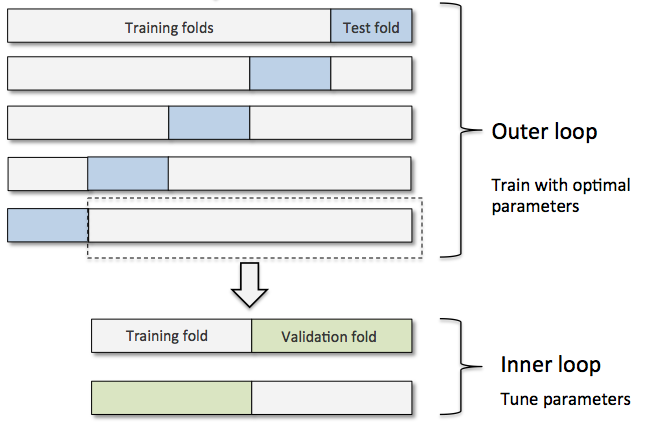
\includegraphics[width=1.0\textwidth]{images/Experimental-validation/nested-crossval.png}
    \caption{Conceptual scheme representing the nested cross validation approach \cite{jacopo_repossi_tutorial_2022}}
    \label{fig:nested-crossval}
\end{figure}

The results will be then compared with the state-of-art results shown in section \ref{subsec:refwork-siena} and then evaluated with respect to the constraints established in the equations \ref{eq:app-constraints}.

\subsection{LSTM Autoencoder} \label{subsec:lstm-exp}
After data extraction and selection, the data will be processed as described in section \ref{subsub:refwork-uab-featext}.

The training phase will be carried out according to the paradigms mentioned in section \ref{subsec:data-grouping}.

For the training phase the following parameters will be used:
\begin{itemize}
    \item batch size of 32
    \item learning rate of 0.001
    \item number of epochs of 150
    \item Adam optimizer 
\end{itemize}

\subsubsection{Patient specific} \label{subsub:patient-specific-exp}
For patient specific, the training phase will be carried out $N$ times, where $N$ is the number of patients considered. Each training phase will involve only the data associated with its patient.

A nested $k_s$-fold cross validation approach will be used, where the test set is 20\% the size of the total data available during the external dataset split and the validation set is 25\% with respect to the remaining data. This gives a test set and validation set of roughly the same size, with the training set being the 60\% of the total data available at each iteration. 

In this case the value chosen for $k_s$ is 5 when possible, down to 3 for patients with the least available data. The test and validation size are scaled accordingly.

Note that the split is applied over the normal instances, as opposed to the single windows, therefore it is possible in some configuration of training, validation and tests, the ratio will not be perfectly balanced at 60\%-20\%-20\%. This fluctuation is considered negligible due to the similar duration of the normal instances of about one hour each.

In the average case, which happens for those patients that have at least 5 normal instances, 20 models ($k_s$ outer splits and, for each one, $k_s-1$ inner splits) will be trained and tested, so the results shown in the next section will be the average of those obtained for each model. 

In each iteration the validation set will be used to find the threshold for the \gls{MSE} reconstruction loss to discriminate anomalous windows from the normal ones.

In the test phase, the test set obtained during the nested cross validation phase, which consists of normal instances that vary depending on the current external fold, will be coupled with all the available seizure instances available for that patient.

\subsubsection{Patient generic} \label{subsub:patient-generic-exp}
For patient generic the training phase will also be carried out $N$ times, where $N$ is the number of patients considered. For each patient the training phase will involve the data associated only with the other patients and tested on the data from the current patient, in a leave-one-patient-out manner.

The training phase will therefore involve data from $N-1$ patients and would be subject to regular $k_g$-fold cross validation as shown in Fig. \ref{fig:leave-one-patient-out}. The validation set would include 20\% of the available data and $k_g$ would be set to 5, which is possible for each patient iteration. The data would be split by patient, meaning that that from a specific patient would be included only in the training set or the validation set, not both.

\begin{figure}[ht]
    \centering
    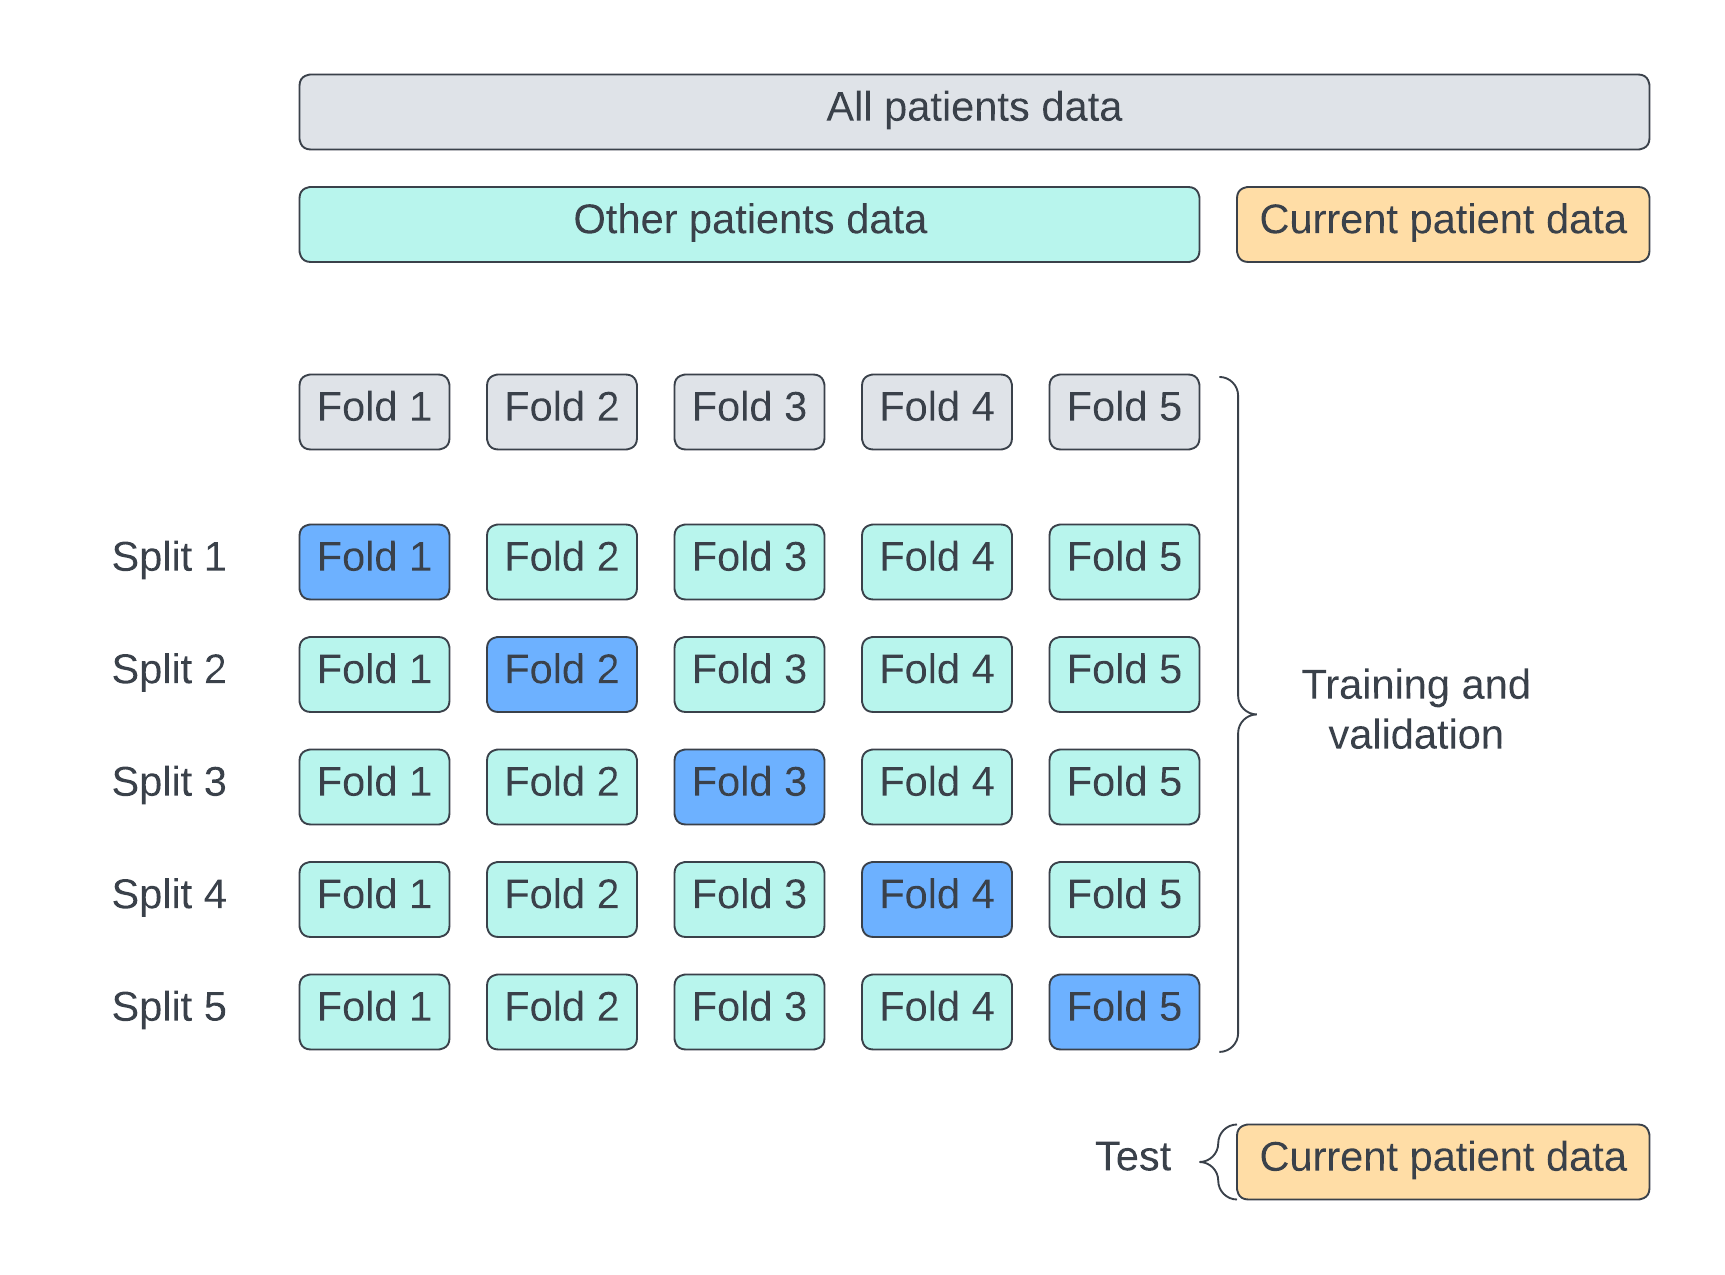
\includegraphics[width=1.0\textwidth]{images/Experimental-validation/leave-one-patient-out.png}
    \caption{Conceptual scheme representing the leave-one-patient-out cross validation approach \cite{jacopo_repossi_tutorial_2022}}
    \label{fig:leave-one-patient-out}
\end{figure}

The test phase will then involve all the data available for the remaining patient and the results shown in the next section will be obtained computing the average performance for each model.

Eventually, for each patient will be created $k_g$ = 5 models, each using much more data than those described in the patient specific approach.

\subsubsection{Inter-patient}  \label{subsub:inter-patient-exp}
Finally, for inter-patient, the training phase presents itself as a follow-up to the previous approach, starting from the model obtained at the end of section  \ref{subsub:patient-generic-exp}, fine-tuning them on the data gathered from the last patient before testing.

The training phase would therefore be carried out $N$ times. For each of the model obtained in section \ref{subsub:patient-generic-exp} a nested $k_s$-fold cross validation will be performed on the data for the associated patient, just as described in section \ref{subsub:patient-specific-exp}.

Different fine-tuning methods are applied, based on the section of the network whose weights would be frozen or reset before the final training phase:

\begin{itemize}
    \item Full fine-tuning, where the whole network would be subject to fine-tuning
    \item Full fine-tuning with last layer reset, where the whole network would be subject to fine-tuning, except for the last dense layer which would be trained from scratch, meaning that its weights would be randomized before fine-tuning
    \item Decoder fine-tuning, where only the second half of the network would be fine-tuned, while the encoder section would see the weights associated to its layers completely frozen
\end{itemize}

Eventually the models obtained at the end of the inter-patient approach would be around 120 for each patient, calculated as the product between the $k_g$ = 5 folds relative to the patient generic approach and the $k_s* (k_s-1)$ with $k_s$ = 5 most of the time, down to 5 when not enough normal instances are available. 

\subsection{CNN and OC-SVM}
After data extraction and selection, the data will be processed as described in section \ref{subsub:refwork-unisa-featext}.

The training phase will be carried out using paradigms similar to those described in section \ref{subsec:lstm-exp}:
ideally the exact same models produced in the work shown in section \ref{subsec:refwork-unisa} would be used, but since those were unavailable the training phase was completely reproduced, obtaining comparable results.

\subsubsection{Original CNN retraining} \label{subsub:original-cnn-retraining}
For the reasons previously explained, the original \gls{CNN} network was trained using regular supervised techniques using the following parameters:

\begin{itemize}
    \item batch size of 1024
    \item learning rate of 0.001
    \item number of epochs of 40
    \item Adam optimizer 
\end{itemize}

Similarly to the patient generic technique described in the previous section, the training phase will involve data from $N-1$ patients and would be subject to regular $k_g$-fold cross validation with $k_g$ = 4. The validation set would include 25\% and be used for hyperparameter optimization, leading to the choice of the parameters mentioned above. Furthermore, differently from the reference work, a \gls{WO} of only 1 second was used in order to reduce the amount of data for training and improve the \gls{IFP} conversion from specificity: with the specificity being equal between two analysis, the reduction in \gls{WO} corresponds to a greater \gls{IFP}.

In this phase a balanced version of the binary cross entropy loss will be used, to address the high imbalance between the two classes, which would otherwise incentivize the network to guess the output as always negative (which is the majority class), independently from the input.

Eventually, for each patient will be created $k_g$ = 4 \gls{CNN} models.

\subsubsection{OC-SVM training}
Similarly to the inter-patient approach described in section \ref{subsub:inter-patient-exp}, the training phase presents itself as a follow-up to the previous approach, starting from the model obtained at the end of section  \ref{subsub:original-cnn-retraining}, extracting the feature extraction section of the network and freezing the weights associated to its layers. For each so obtained feature extractor, a regular $k_s$-fold cross validation would be applied to train a \gls{OC-SVM} network over the data belonging to the current patient, with $k_s$ ranging between 5 and 3 just as described in section \ref{subsub:inter-patient-exp}.

The \gls{OC-SVM} model would have to learn the meaning of normality over the embeddings computed from the patient data extracted by the feature extractor.

This would simulate the real-life scenario where a certain amount of seizure and normal instances is gathered for many patients and used to train a complex network that would successively be paired to a simpler unsupervised anomaly detector which would, supposedly in a couple of hours, be able to fit the specific embedded representation of the brain activity for such patient. 

The parameters used for the \gls{OC-SVM} were manually tested and optimized to maximize the specificity, leading to the following configuration:

\begin{itemize}
    \item nu of 0.01
    \item kernel "\gls{RBF}"
    \item gamma "scale"
\end{itemize}

The specific implementation of \gls{OC-SVM} is available at \cite{noauthor_sklearnsvmoneclasssvm_nodate}.

Eventually the models obtained at the end of this training phase would be around 20 for each patient, calculated as the product between the $k_g$ = 4 folds relative to the patient generic approach and the $k_s$, following the considerations discussed above. 


\section{Description of the data and the case studies used for the experimentation}
The data used was described in section \ref{subsec:dataset-used} and the relative selection and processing were shown in section \ref{subsub:refwork-uab-featext} and \ref{subsub:refwork-unisa-featext}, depending on the model.

In Fig. \ref{fig:raw-edf} an example of raw signal is shown, while in Figs. \ref{fig:lstm-processed-edf} and \ref{fig:spectrogram-processed-edf} the processed signals for respectively \gls{LSTM} and \gls{CNN} based models are shown. 

\begin{figure}[ht]
    \centering
    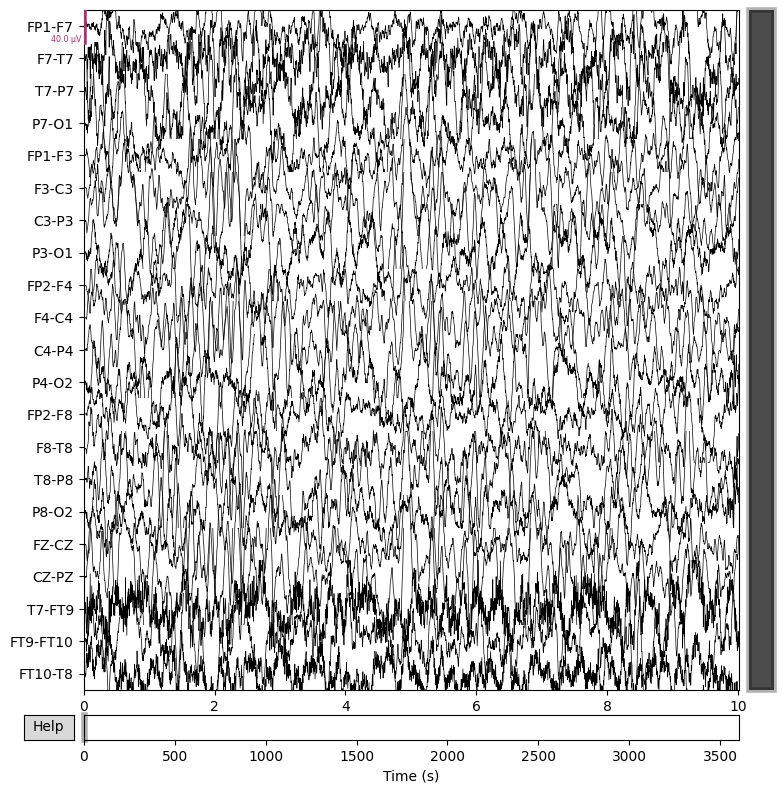
\includegraphics[width=0.75\textwidth]{images/Experimental-validation/raw-edf.png}
    \caption{10 seconds example of raw signal}
    \label{fig:raw-edf}
\end{figure}

\begin{figure}[ht]
    \centering
    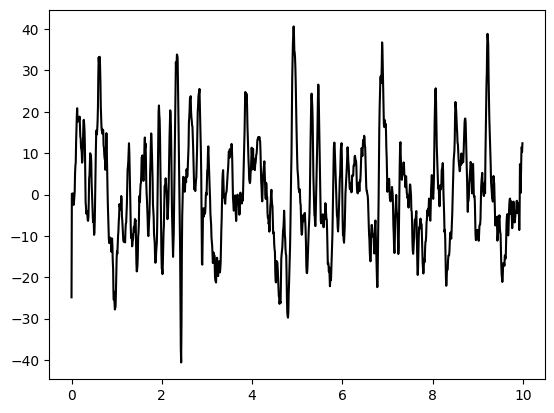
\includegraphics[width=0.5\textwidth]{images/Experimental-validation/lstm-processed-edf.png}
    \caption{Single window at the end of processing for LSTM based models}
    \label{fig:lstm-processed-edf}
\end{figure}

\begin{figure}[ht]
    \centering
    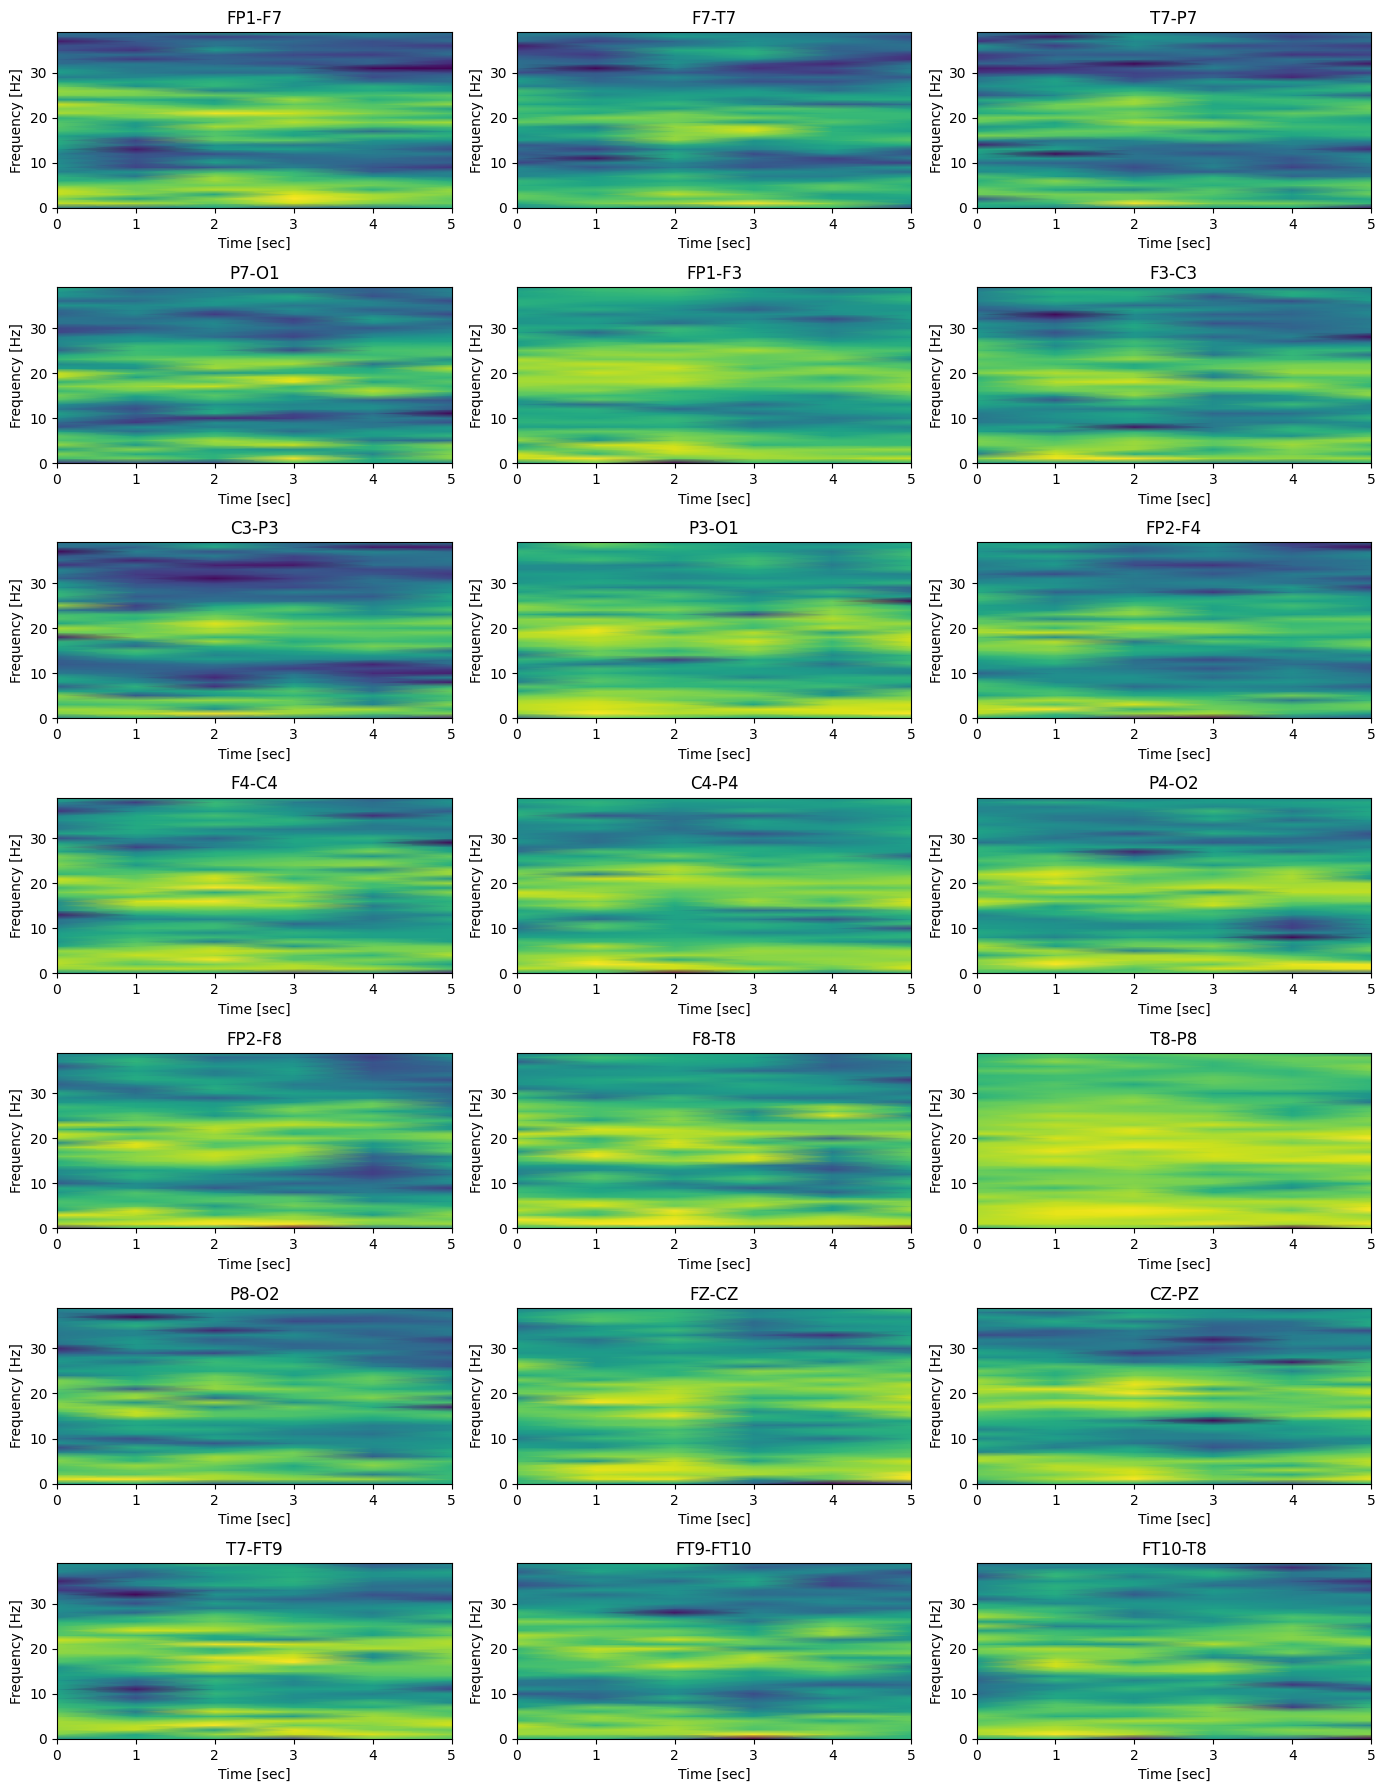
\includegraphics[width=1.0\textwidth]{images/Experimental-validation/spectrogram-processed-edf.png}
    \caption{Single window at the end of processing for CNN based models}
    \label{fig:spectrogram-processed-edf}
\end{figure}

\clearpage
\section{Presentation and analysis of the results}

\subsection{Result tables}

\subsubsection{LSTM autoencoder}
The first results to be presented will concern the \gls{LSTM} autoencoder network.

\begin{table}[ht]
    \centering
    \begin{tabular}{c|rrrrr}
    Pat.  & $pred\%$ & $spec\%$ & $\overline{t}_p$   & $t_p^m$  & $t_p^M$   \\ \hline
    chb01   & 37.9   & 99.9   & 930.5   & 205.3   & 1876.8  \\
    chb02   & 100.0  & 99.8   & 2432.2  & 1570.7  & 3293.7  \\
    chb03   & 6.4    & 99.9   & 448.7   & 172.3   & 725.0   \\
    chb04   & 25.0   & 91.9   & 7232.0  & 6796.0  & 7668.0  \\
    chb05   & 30.0   & 98.3   & 1089.4  & 465.2   & 1939.8  \\
    chb06   & 25.5   & 100.0  & 3949.4  & 1651.2  & 6568.6  \\
    chb07   & 61.1   & 99.8   & 5307.0  & 1024.0  & 10381.0 \\
    chb08   & 67.0   & 99.9   & 1651.8  & 971.0   & 2216.9  \\
    chb09   & 58.3   & 85.2   & 8420.7  & 5535.3  & 12034.0 \\
    chb10   & 57.1   & 99.9   & 4443.7  & 3019.2  & 6499.2  \\
    chb11   & 16.7   & 99.7   & 859.0   & 859.0   & 859.0   \\
    chb12   & 11.5   & 100.0  & 654.8   & 537.5   & 778.1   \\
    chb13   & 27.1   & 99.9   & 1326.1  & 712.5   & 1828.0  \\
    chb14   & 55.6   & 99.9   & 1668.0  & 234.8   & 3140.9  \\
    chb15   & 28.8   & 99.7   & 873.4   & 373.7   & 2216.0  \\
    chb16   & 24.0   & 99.2   & 792.1   & 714.5   & 877.1   \\
    chb17   & 33.3   & 99.5   & 1016.0  & 873.0   & 1255.5  \\
    chb18   & 59.2   & 99.4   & 1552.2  & 683.6   & 2014.3  \\
    chb19   & 83.3   & 99.7   & 2763.7  & 2451.3  & 3076.0  \\
    chb20   & 16.0   & 99.6   & 1475.6  & 1454.5  & 1496.7  \\
    chb21   & 45.8   & 99.7   & 1861.9  & 985.0   & 2405.0  \\
    chb22   & 27.8   & 99.9   & 1842.7  & 1182.0  & 2503.3  \\
    chb23   & 30.6   & 99.9   & 1183.1  & 735.5   & 1828.0  \\
    chb24   & 8.3    & 99.8   & 1570.9  & 854.0   & 2531.3  \\ \hline
    Av.     & 39.0   & 98.8   & 2306.0  & 1419.2  & 3333.8  \\ \hline
    \end{tabular}
    \caption{Patient specific instance-wise performance of LSTM autoencoder network on \glsentrylong{CHB-MIT} dataset}
    \label{tab:patient-specific-lstm-instance} 
\end{table}

In the patient specific scenario, which results are shown in Table \ref{tab:patient-specific-lstm-instance}, the average $pred\%$ is about 39.0\%, which is quite low when compared to the reference works with average prediction accuracy of 100\%, but that is to be expected since the training was optimized to maximize the specificity. In fact, it could not have been otherwise: since the only data available during the training phase was theoretically made only by normal instances, optimizing the results to maximize the prediction accuracy as the reference works supposedly did, was indeed not an option at all.

In this case the average $spec\%$ was 98.8\%, which is higher than the 98.0\% from the patient specific analysis in \gls{UNISA}'s work from section \ref{subsec:refwork-unisa}, but with a lower \gls{WD} the current \gls{LSTM} network's specificity translates in a lower \gls{IFP} of 161.5 seconds, as opposed to 296 seconds.

The average $t_p^m$ is about 1419 seconds, which is definitely enough time for the patient to adopt safety measures for the incoming epileptic seizure.

The average $\overline{t}_w\%$ and the average $t_w^M$ are respectively 1428\% and 2064\%, highlighting the immense differences between the prediction times and the \gls{IFP}, thus making the system simply unusable.

\begin{table}[ht]
    \centering
    \begin{tabular}{c|rrrrr}
    Pat.  & $pred\%$ & $spec\%$ & $\overline{t}_p$   & $t_p^m$  & $t_p^M$   \\ \hline
    chb01   & 0.0    & 100.0  &         &         &         \\
    chb02   & 50.0   & 100.0  & 1300.8  & 1223.5  & 1378.0  \\
    chb03   & 0.0    & 100.0  &         &         &         \\
    chb04   & 20.0   & 98.3   & 7596.5  & 7596.5  & 7596.5  \\
    chb05   & 0.0    & 100.0  &         &         &         \\
    chb06   & 2.0    & 100.0  & 1602.0  & 1602.0  & 1602.0  \\
    chb07   & 0.0    & 99.9   &         &         &         \\
    chb08   & 0.0    & 100.0  &         &         &         \\
    chb09   & 25.0   & 91.7   & 11587.2 & 11587.2 & 11587.2 \\
    chb10   & 14.3   & 100.0  & 3404.8  & 3404.8  & 3404.8  \\
    chb11   & 0.0    & 100.0  &         &         &         \\
    chb12   & 0.0    & 100.0  &         &         &         \\
    chb13   & 0.0    & 100.0  &         &         &         \\
    chb14   & 0.0    & 100.0  &         &         &         \\
    chb15   & 0.0    & 100.0  &         &         &         \\
    chb16   & 0.0    & 100.0  &         &         &         \\
    chb17   & 0.0    & 100.0  &         &         &         \\
    chb18   & 3.3    & 100.0  & 938.0   & 938.0   & 938.0   \\
    chb19   & 0.0    & 100.0  &         &         &         \\
    chb20   & 0.0    & 99.9   &         &         &         \\
    chb21   & 0.0    & 100.0  &         &         &         \\
    chb22   & 0.0    & 100.0  &         &         &         \\
    chb23   & 0.0    & 100.0  &         &         &         \\
    chb24   & 1.7    & 100.0  & 854.0   & 854.0   & 854.0   \\ \hline
    Av.     & 4.8    & 99.6   & 3897.6  & 3886.6  & 3908.6  \\ \hline
    \end{tabular}
    \caption{Patient generic instance-wise performance of LSTM autoencoder network with 100 percentile on validation set threshold on \glsentrylong{CHB-MIT} dataset}
    \label{tab:patient-generic-100perc-lstm-instance} 
\end{table}

The results concerning the patient generic scenario are reported in Table \ref{tab:patient-generic-100perc-lstm-instance}. 
The average $pred\%$ is about 4.8\%, meaning that the network almost completely fails to predict incoming epileptic seizures.
For many patients, not even one single positive detection can be observed, making the task of computing the prediction times meaningless.

Of course the average $spec\%$ is way higher than the patient specific one, but given that the prediction accuracy is so low it's not even worth considering.

The reason for such a low prediction accuracy can be attributed to the higher amount of training and validation data, which leads the validation set to inevitably contain many more outlier (but still normal) cases. Therefore choosing the 100th percentile on the validation set as the threshold could be a sub-optimal strategy.


\begin{table}[ht]
    \centering
    \begin{tabular}{c|rrrrr}
    Pat.  & $pred\%$ & $spec\%$ & $\overline{t}_p$   & $t_p^m$  & $t_p^M$   \\ \hline
    chb01   & 2.9    & 99.9   & 210.0   & 210.0   & 210.0   \\
    chb02   & 70.0   & 100.0  & 1805.8  & 1714.8  & 1896.8  \\
    chb03   & 0.0    & 100.0  &         &         &         \\
    chb04   & 30.0   & 91.3   & 7344.0  & 7039.6  & 7648.4  \\
    chb05   & 0.0    & 99.9   &         &         &         \\
    chb06   & 16.0   & 100.0  & 2764.1  & 1379.3  & 4755.3  \\
    chb07   & 26.7   & 99.5   & 7725.3  & 5719.0  & 10575.0 \\
    chb08   & 0.0    & 100.0  &         &         &         \\
    chb09   & 40.0   & 65.3   & 9916.1  & 8233.6  & 12181.2 \\
    chb10   & 20.0   & 100.0  & 4579.9  & 4020.0  & 5350.0  \\
    chb11   & 0.0    & 100.0  &         &         &         \\
    chb12   & 0.0    & 100.0  &         &         &         \\
    chb13   & 7.5    & 100.0  & 569.5   & 150.0   & 989.0   \\
    chb14   & 5.0    & 100.0  & 2600.0  & 2600.0  & 2600.0  \\
    chb15   & 0.0    & 100.0  &         &         &         \\
    chb16   & 16.0   & 99.0   & 604.0   & 543.3   & 664.7   \\
    chb17   & 6.7    & 99.8   & 828.0   & 828.0   & 828.0   \\
    chb18   & 16.7   & 100.0  & 1252.0  & 1147.3  & 1348.7  \\
    chb19   & 0.0    & 100.0  &         &         &         \\
    chb20   & 4.0    & 99.8   & 1010.0  & 1010.0  & 1010.0  \\
    chb21   & 15.0   & 100.0  & 1802.0  & 602.0   & 2604.0  \\
    chb22   & 13.3   & 99.8   & 2029.0  & 1182.0  & 2876.0  \\
    chb23   & 0.0    & 100.0  &         &         &         \\
    chb24   & 16.7   & 99.8   & 1491.9  & 854.0   & 2134.0  \\ \hline
    Av.     & 12.8   & 98.1   & 2908.2  & 2327.1  & 3604.4  \\ \hline
    \end{tabular}
    \caption{Patient generic instance-wise performance of LSTM autoencoder network with 99.9 percentile on validation set threshold on \glsentrylong{CHB-MIT} dataset}
    \label{tab:patient-generic-99.9perc-lstm-instance} 
\end{table}

In Table \ref{tab:patient-generic-99.9perc-lstm-instance} the results for the patient generic analysis are reported, where the threshold is chosen to be the 99.9th percentile of the validation set, with the idea of reaching a similar value of $spec\%$ to make the results more comparable.

The $spec\%$ is about 98.1\%, which is in fact lower than the previous case, as expected. It is even lower than the specificity in the patient specific case, but so is the average $pred\%$: at a value of about 12.8\%, compared to the 39.0\% of the patient specific, it's clear that the patient generic approach leads to worse results overall.

\begin{table}[ht]
    \centering
    \begin{tabular}{c|rrrrr}
    Pat.  & $pred\%$ & $spec\%$ & $\overline{t}_p$   & $t_p^m$  & $t_p^M$   \\ \hline
    chb01   & 14.3   & 99.7   & 685.3   & 210.0   & 1160.7  \\
    chb02   & 80.0   & 100.0  & 2256.6  & 2148.4  & 2364.8  \\
    chb03   & 0.0    & 99.9   &         &         &         \\
    chb04   & 40.0   & 90.0   & 6811.6  & 5973.2  & 7650.0  \\
    chb05   & 4.0    & 99.8   & 1828.0  & 1828.0  & 1828.0  \\
    chb06   & 42.0   & 99.9   & 3953.2  & 1128.7  & 9021.3  \\
    chb07   & 60.0   & 99.2   & 5436.2  & 1914.7  & 11175.3 \\
    chb08   & 16.0   & 100.0  & 2029.5  & 1524.0  & 2535.0  \\
    chb09   & 65.0   & 65.3   & 7557.4  & 4648.0  & 12181.2 \\
    chb10   & 37.1   & 100.0  & 3825.6  & 3030.4  & 5350.4  \\
    chb11   & 10.0   & 99.8   & 1146.0  & 1146.0  & 1146.0  \\
    chb12   & 0.0    & 100.0  &         &         &         \\
    chb13   & 27.5   & 100.0  & 1265.0  & 188.0   & 2809.3  \\
    chb14   & 20.0   & 100.0  & 1954.2  & 1230.0  & 2664.7  \\
    chb15   & 0.0    & 100.0  &         &         &         \\
    chb16   & 28.0   & 97.7   & 1190.0  & 974.7   & 1412.7  \\
    chb17   & 20.0   & 99.7   & 841.5   & 828.0   & 855.0   \\
    chb18   & 26.7   & 100.0  & 1668.1  & 1254.7  & 2046.7  \\
    chb19   & 10.0   & 100.0  & 2364.0  & 2364.0  & 2364.0  \\
    chb20   & 8.0    & 99.7   & 1010.0  & 1010.0  & 1010.0  \\
    chb21   & 30.0   & 99.9   & 1593.3  & 1136.0  & 1918.0  \\
    chb22   & 13.3   & 99.6   & 2033.0  & 1182.0  & 2884.0  \\
    chb23   & 3.3    & 100.0  & 1304.0  & 1304.0  & 1304.0  \\
    chb24   & 25.0   & 99.7   & 1653.6  & 854.0   & 2740.0  \\ \hline
    Av.     & 24.2   & 97.9   & 2495.5  & 1708.4  & 3639.1  \\ \hline
    \end{tabular}
    \caption{Patient generic instance-wise performance of LSTM autoencoder network with 99.8 percentile on validation set threshold on \glsentrylong{CHB-MIT} dataset}
    \label{tab:patient-generic-99.8perc-lstm-instance} 
\end{table}

In Table \ref{tab:patient-generic-99.8perc-lstm-instance} the results of an other analysis with an even lower percentile value for the threshold (99.8th percentile) is shown.

The average $spec\%$ is even lower, but the resulting increase in the average $perc\%$ is still not enough to reach the patient specific's average $pred\%$ (97.9\% in patient generic with 99.8th percentile vs 39.0\% in patient specific).

Overall in the three patient generic results analyzed, only the 100th percentile ones had improvements on the $\overline{t}_w$ and $t_w^M$, but the close-to-zero average $pred\%$ makes them not worth considering. The 99.9th and 99.8th percentile, instead, are comparatively worse all across the board.

It is also clear that the analysis with lower values of the percentiles is statistically biased, in that it relies on observations on the test set. Being presented only for illustration purposes, it's deemed incorrect to even consider improving the models that produced those results, therefore they will not be used as starting point for the inter-patient approach.

\begin{table}[ht]
    \centering
    \begin{tabular}{c|rrrrr}
    Pat.  & $pred\%$ & $spec\%$ & $\overline{t}_p$   & $t_p^m$  & $t_p^M$   \\ \hline
    chb01   & 28.7   & 99.5   & 596.3   & 241.8   & 1011.8  \\
    chb02   & 100.0  & 99.1   & 3095.5  & 2875.7  & 3315.3  \\
    chb03   & 8.1    & 99.8   & 582.6   & 175.4   & 1152.3  \\
    chb04   & 25.8   & 93.3   & 7063.7  & 6495.7  & 7631.6  \\
    chb05   & 20.6   & 98.8   & 1135.8  & 367.6   & 1964.1  \\
    chb06   & 27.2   & 99.9   & 3838.8  & 1710.3  & 6128.8  \\
    chb07   & 50.0   & 99.2   & 4004.8  & 1622.9  & 7279.4  \\
    chb08   & 72.4   & 99.9   & 1774.5  & 851.5   & 2471.8  \\
    chb09   & 62.5   & 76.2   & 8410.4  & 5766.7  & 12149.5 \\
    chb10   & 56.6   & 99.9   & 4585.2  & 3078.5  & 6593.5  \\
    chb11   & 60.0   & 97.3   & 1125.2  & 837.6   & 1412.7  \\
    chb12   & 11.4   & 100.0  & 554.0   & 415.0   & 699.5   \\
    chb13   & 45.6   & 99.9   & 1328.2  & 181.3   & 2848.6  \\
    chb14   & 52.2   & 99.9   & 1668.1  & 568.7   & 2831.0  \\
    chb15   & 24.7   & 99.8   & 870.1   & 181.0   & 2481.7  \\
    chb16   & 17.8   & 99.3   & 782.0   & 755.7   & 808.3   \\
    chb17   & 23.3   & 99.5   & 1305.7  & 1170.1  & 1441.3  \\
    chb18   & 57.0   & 99.4   & 1704.1  & 1077.0  & 2156.7  \\
    chb19   & 76.7   & 99.6   & 2589.2  & 2107.5  & 3070.8  \\
    chb20   & 16.6   & 99.6   & 1544.4  & 1529.2  & 1559.7  \\
    chb21   & 58.8   & 99.6   & 1831.0  & 914.7   & 2530.2  \\
    chb22   & 14.4   & 99.9   & 1417.1  & 1023.8  & 1917.2  \\
    chb23   & 25.6   & 100.0  & 1365.3  & 828.6   & 1854.5  \\
    chb24   & 13.0   & 99.8   & 1498.7  & 944.6   & 2093.1  \\ \hline
    Av.     & 39.5   & 98.3   & 2277.9  & 1488.4  & 3225.1  \\ \hline
    \end{tabular}
    \caption{Fully fine-tuned inter-patient instance-wise performance of LSTM autoencoder network on \glsentrylong{CHB-MIT} dataset}
    \label{tab:full-inter-patient-lstm-instance} 
\end{table}

In Table \ref{tab:full-inter-patient-lstm-instance} the inter-patient results are presented. The starting point of this training was the set of models that produced the results in Table \ref{tab:patient-generic-100perc-lstm-instance}.

The average $pred\%$ is about 39.5\%, which is pretty close to the average $pred\%$ of 39.0\% from the patient specific case, however the average $spec\%$, at 98.3\% is significantly lower when compared to 98.8\% for patient specific. 

Note that even tho the both the $pred\%$ and $spec\%$ difference in values is 0.5\%, the variation in the second case is considered to be significant for two reasons: as stated before the training has to maximize $spec\%$, making the relative improvements way more appreciated, and slight increases of $spec\%$ when close to 100\% lead to far higher values of $IFP$.

Also the values of $\overline{t}_w$ and $t_w^M$ are worse, at respectively 1950\% and 2761\% compared to 1428\% and 2064\% for the patient specific case.

Despite the fact that the patient specific results are closer to the inter-patient ones than the patient generic, the inter-patient results are still objectively worse. Improvements may be achieved by varying the fine-tuning techniques.

\begin{table}[ht]
    \centering
    \begin{tabular}{c|rrrrr}
    Pat.  & $pred\%$ & $spec\%$ & $\overline{t}_p$   & $t_p^m$  & $t_p^M$   \\ \hline
    chb01   & 31.4   & 99.8   & 788.0   & 241.8   & 1403.4  \\
    chb02   & 100.0  & 99.4   & 2775.8  & 2244.9  & 3306.7  \\
    chb03   & 6.9    & 99.7   & 458.5   & 131.5   & 809.6   \\
    chb04   & 25.0   & 92.5   & 7093.2  & 6539.3  & 7647.2  \\
    chb05   & 25.0   & 98.7   & 1057.7  & 411.2   & 1791.2  \\
    chb06   & 27.4   & 99.9   & 3670.0  & 1779.9  & 5637.3  \\
    chb07   & 38.9   & 99.5   & 6698.6  & 3857.4  & 9987.4  \\
    chb08   & 66.0   & 99.9   & 1739.2  & 1039.5  & 2284.0  \\
    chb09   & 58.3   & 76.4   & 8451.0  & 5573.1  & 12077.6 \\
    chb10   & 56.9   & 99.9   & 4447.4  & 3002.0  & 6528.6  \\
    chb11   & 18.3   & 99.6   & 789.8   & 771.4   & 808.2   \\
    chb12   & 9.4    & 100.0  & 627.9   & 573.2   & 683.0   \\
    chb13   & 32.3   & 99.9   & 1167.9  & 308.3   & 2151.3  \\
    chb14   & 53.2   & 99.9   & 1893.5  & 631.2   & 3181.2  \\
    chb15   & 26.6   & 99.8   & 892.4   & 273.3   & 2358.9  \\
    chb16   & 19.6   & 98.9   & 811.0   & 739.2   & 882.1   \\
    chb17   & 21.1   & 99.4   & 1281.4  & 1281.4  & 1281.4  \\
    chb18   & 59.3   & 98.9   & 1678.2  & 1071.7  & 2146.3  \\
    chb19   & 81.7   & 99.3   & 2823.3  & 2562.7  & 3083.9  \\
    chb20   & 15.0   & 99.6   & 1482.9  & 1482.9  & 1482.9  \\
    chb21   & 62.1   & 99.6   & 1771.4  & 947.7   & 2394.8  \\
    chb22   & 16.7   & 99.9   & 1902.7  & 1542.4  & 2263.1  \\
    chb23   & 23.3   & 100.0  & 1192.5  & 957.2   & 1471.8  \\
    chb24   & 11.1   & 99.8   & 1499.6  & 891.5   & 2212.7  \\ \hline
    Av.     & 36.9   & 98.3   & 2374.8  & 1618.9  & 3244.8  \\ \hline
    \end{tabular}
    \caption{Fully fine-tuned with last layer reset inter-patient instance-wise performance of LSTM autoencoder network on \glsentrylong{CHB-MIT} dataset}
    \label{tab:reset-inter-patient-lstm-instance} 
\end{table}

In Table \ref{tab:reset-inter-patient-lstm-instance} the results are presented for the inter-patient where the source model is fully fine-tuned after resetting the parameters in the last layer.

The average $pred\%$ is 36.9 and the average $spec\%$ is 98.3. Also the $\overline{t}_w\%$ and $t_w^M$  of 1974\% are 2697\% are pretty similar to the previous scenario. Overall, only the $pred\%$ is slightly lower, meaning that this approach did not lead to noticeable improvements, if any.

\begin{table}[ht]
    \centering
    \begin{tabular}{c|rrrrr}
    Pat.  & $pred\%$ & $spec\%$ & $\overline{t}_p$   & $t_p^m$  & $t_p^M$   \\ \hline
    chb01   & 31.7   & 99.6   & 906.4   & 260.3   & 1625.3  \\
    chb02   & 100.0  & 99.4   & 2887.0  & 2463.1  & 3310.9  \\
    chb03   & 5.6    & 99.7   & 436.1   & 238.4   & 678.0   \\
    chb04   & 25.8   & 92.3   & 7005.0  & 6295.1  & 7647.3  \\
    chb05   & 20.6   & 98.8   & 1089.3  & 348.1   & 1974.1  \\
    chb06   & 24.5   & 99.9   & 3971.1  & 2169.0  & 6176.4  \\
    chb07   & 40.0   & 99.6   & 7135.1  & 4162.2  & 10380.4 \\
    chb08   & 64.4   & 99.9   & 1664.7  & 908.2   & 2234.0  \\
    chb09   & 58.3   & 76.6   & 8503.4  & 5674.5  & 12079.4 \\
    chb10   & 56.4   & 99.9   & 4379.0  & 3003.1  & 6520.9  \\
    chb11   & 31.7   & 99.4   & 979.3   & 940.8   & 1017.8  \\
    chb12   & 8.0    & 100.0  & 580.0   & 580.0   & 580.0   \\
    chb13   & 31.5   & 99.9   & 1120.4  & 228.3   & 2120.2  \\
    chb14   & 49.4   & 99.9   & 1856.0  & 595.6   & 3151.3  \\
    chb15   & 21.8   & 99.8   & 957.7   & 239.1   & 2456.1  \\
    chb16   & 15.6   & 99.0   & 771.3   & 748.3   & 792.0   \\
    chb17   & 21.1   & 99.4   & 1206.2  & 1206.2  & 1206.2  \\
    chb18   & 57.8   & 99.0   & 1677.7  & 1057.2  & 2103.9  \\
    chb19   & 83.3   & 99.2   & 2774.5  & 2455.7  & 3093.2  \\
    chb20   & 15.8   & 99.6   & 1443.7  & 1443.7  & 1443.7  \\
    chb21   & 63.3   & 99.5   & 1816.8  & 858.6   & 2457.3  \\
    chb22   & 15.6   & 99.8   & 1925.2  & 1182.0  & 2668.5  \\
    chb23   & 23.3   & 99.9   & 1112.7  & 906.6   & 1263.2  \\
    chb24   & 10.0   & 99.8   & 1547.5  & 946.4   & 2270.6  \\ \hline
    Av.     & 36.5   & 98.3   & 2406.1  & 1621.3  & 3302.1  \\ \hline
    \end{tabular}
    \caption{Decoder fine-tuned inter-patient instance-wise performance of LSTM autoencoder network on \glsentrylong{CHB-MIT} dataset}
    \label{tab:decoder-inter-patient-lstm-instance} 
\end{table}

In Table \ref{tab:decoder-inter-patient-lstm-instance} the results are presented for the inter-patient where the parameters for the layers in the first half of the source model, which is to say the encoder part, are frozen; the second half of the source model is instead fine-tuned as usual.

The average $pred\%$ is 36.5, the average $spec\%$ is 98.3, the $\overline{t}_w\%$ and $t_w^M$ are 1997\% and 2740\%.

Just like the previous case, also this time the results are close without any noticeable improvement.


\subsubsection{CNN and OC-SVM}
Finally, the results of the \gls{OC-SVM} training is reported in Table \ref{tab:cnn-ocsvm-instance}.

Even if the hyper-parameters were optimized to maximize the specificity, only an average value of about 96.3\% is reached, but the $pred\%$ is far higher the one presented in Table \ref{tab:patient-specific-lstm-instance} (76.7\% vs 39.0\%).

Despite the average $spec\%$ being substantially lower than the patient specific case presented before, thanks to the bigger \gls{WD}, the $\overline{t}_w\%$ is still comparable, at a value of 1701\%. The same can not be stated for $t_w^M$,  with a value of 2936\%.

\begin{table}[ht]
    \centering
    \begin{tabular}{c|rrrrr}
    Pat.  & $pred\%$ & $spec\%$ & $\overline{t}_p$   & $t_p^m$  & $t_p^M$   \\ \hline
    chb01   & 27.9   & 97.6   & 1052.9  & 658.9   & 1545.4  \\
    chb02   & 87.5   & 96.5   & 1561.2  & 1197.9  & 1924.6  \\
    chb03   & 51.4   & 96.6   & 1277.1  & 497.5   & 2007.8  \\
    chb04   & 77.1   & 96.4   & 3926.2  & 870.8   & 7692.5  \\
    chb05   & 83.0   & 97.7   & 1304.0  & 423.2   & 2006.8  \\
    chb06   & 92.5   & 98.6   & 4980.3  & 41.0    & 10098.0 \\
    chb07   & 77.8   & 90.5   & 7590.0  & 3787.1  & 12119.2 \\
    chb08   & 100.0  & 98.5   & 2182.6  & 1630.0  & 2793.8  \\
    chb09   & 97.9   & 78.8   & 6020.9  & 2022.9  & 12099.6 \\
    chb10   & 99.3   & 98.8   & 3278.4  & 595.0   & 6759.8  \\
    chb11   & 100.0  & 98.3   & 1937.7  & 1209.2  & 2666.2  \\
    chb12   & 90.0   & 98.5   & 1077.5  & 236.0   & 2335.2  \\
    chb13   & 91.4   & 92.9   & 1291.6  & 391.9   & 3251.6  \\
    chb14   & 85.0   & 98.8   & 1579.0  & 531.5   & 3120.0  \\
    chb15   & 57.3   & 98.9   & 998.3   & 219.0   & 2495.0  \\
    chb16   & 65.0   & 95.1   & 1200.8  & 495.0   & 1957.8  \\
    chb17   & 72.2   & 93.7   & 2087.4  & 1412.9  & 2682.5  \\
    chb18   & 100.0  & 98.5   & 1563.7  & 193.5   & 3098.5  \\
    chb19   & 95.8   & 95.7   & 2526.5  & 2170.0  & 2882.9  \\
    chb20   & 40.0   & 98.7   & 1059.0  & 846.9   & 1289.2  \\
    chb21   & 34.4   & 98.3   & 1537.2  & 1050.5  & 1996.0  \\
    chb22   & 77.8   & 98.6   & 1761.4  & 985.0   & 2531.7  \\
    chb23   & 90.3   & 97.1   & 1825.9  & 222.1   & 3259.2  \\
    chb24   & 47.5   & 98.4   & 1683.3  & 544.5   & 2865.2  \\ \hline
    Av.     & 76.7   & 96.3   & 2304.3  & 926.4   & 3978.3  \\ \hline
    \end{tabular}
    \caption{OC-SVM patient specific with pre-trained patient generic CNN instance-wise performance on \glsentrylong{CHB-MIT} dataset}
    \label{tab:cnn-ocsvm-instance} 
\end{table}

Overall the performance of the models in Table \ref{tab:patient-specific-lstm-instance} have different strengths when compared to those from the patient specific case, even if the stated focus on optimizing the specificity suggests that is may still be arguably worse.

Regardless of such performance with respect to the patient specific scenario, the model is still far worse than the reference works presented in sections \ref{subsec:refwork-siena} and \ref{subsec:refwork-unisa}.

\clearpage
\subsection{Overall comparison}
Now a more transversal analysis will be presented, taking into account the single metrics with their respective variance also including the performance registered for the reference works. The analysis will be carried out through boxplots, considering the variance of each performance metric across the patients results.

\begin{figure}[ht]
    \centering
    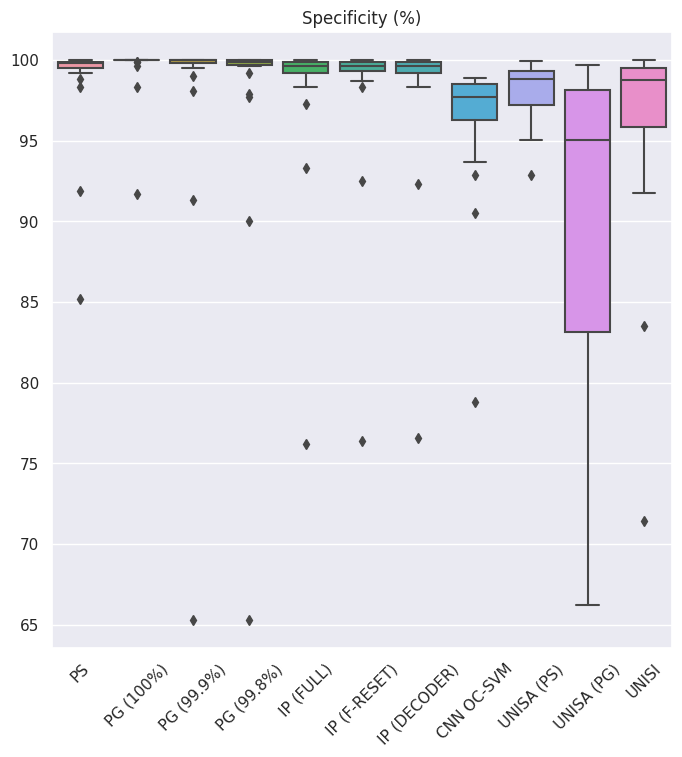
\includegraphics[width=1.0\textwidth]{images/Experimental-validation/boxplot_spec.png}
    \caption{Boxplot comparison of specificity (\%)}
    \label{fig:boxplot_spec}
\end{figure}
In Fig. \ref{fig:boxplot_spec} the comparison for $spec\%$ is shown. The top performers are the \gls{LSTM} based models, while the the \gls{CNN} \gls{OC-SVM} one falls even behind the reference works. Among those reference works, the specificity from the UNISA's patient specific work is the best, with comparable results from the \gls{UNISI} one.

It should be noted that the difference between the \gls{LSTM} based systems and the other ones is less significant than what appears at a glance, because its applicability is conditioned by the \gls{WD} and \gls{WO} values: as stated, to higher values of \gls{WD} with the same $spec\%$ correspond higher values of \gls{IFP}, therefore increasing the $\overline{t}_w\%$ and $t_w^M$ which are, ultimately, the values to optimize.

For reference, every system that is \gls{LSTM} based has a \gls{WD} of 2 seconds, while the others use a \gls{WD} of 6 seconds.

\begin{figure}[ht]
    \centering
    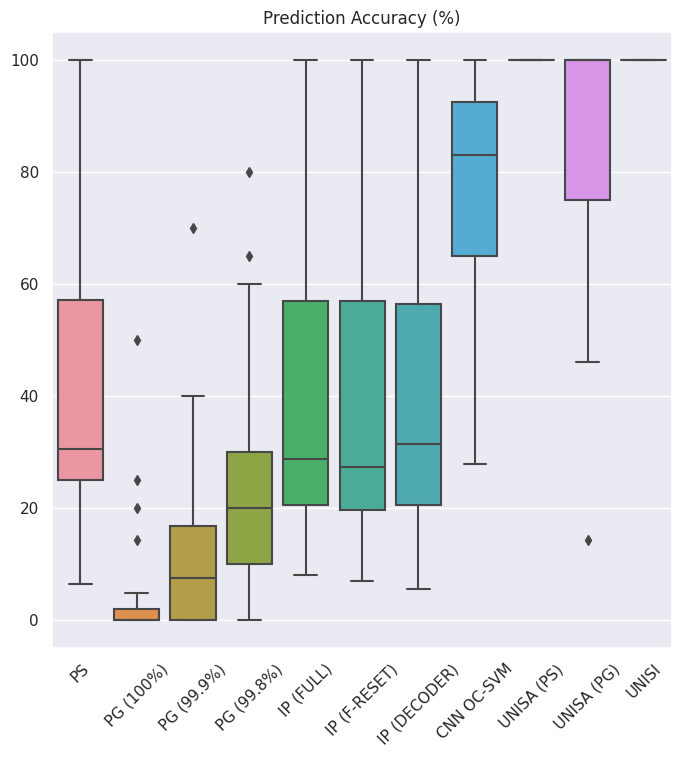
\includegraphics[width=1.0\textwidth]{images/Experimental-validation/boxplot_pred.png}
    \caption{Boxplot comparison of prediction accuracy (\%)}
    \label{fig:boxplot_pred}
\end{figure}

The comparison for $pred\%$ is shown in Fig. \ref{fig:boxplot_pred}. The patient specific reference works achieve a straight 100\% with 0 variance. Among the reference works, the UNISA's patient generic one has the worst value of $pred\%$, but is still higher than any of the systems trained in this thesis.

Among the system trained, the best $pred\%$ is reached for the \gls{CNN} \gls{OC-SVM}, which is of course based on the patient generic \gls{UNISA}'s architecture, which was subject to an initial supervised training procedure.

Close-to-zero values of $pred\%$ are achieved by the \gls{LSTM} based system trained with the patient generic approach using the most limiting threshold criterion, while the best results are reached for those works whose last (or only) approach used for training was the patient specific one.

\begin{figure}[ht]
    \centering
    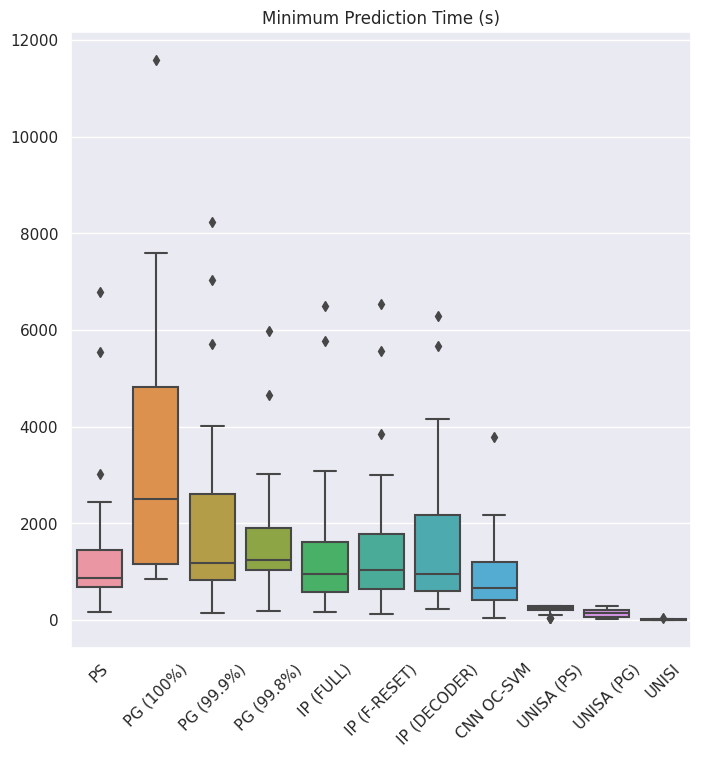
\includegraphics[width=1.0\textwidth]{images/Experimental-validation/boxplot_mPT.png}
    \caption{Boxplot comparison of Minimum Prediction Time (s)}
    \label{fig:boxplot_mPT}
\end{figure}

In the minimum prediction times department, compared in Fig. \ref{fig:boxplot_mPT}, unacceptable values for real-life use are achieved for \gls{UNISI}'s and patient generic \gls{UNISA}'s works, while the patient specific \gls{UNISA} one reach times that starts to be acceptable, while still being on the low side.

Every \gls{LSTM} based system obtains minimum prediction times that are way too high, particularly for the 100th percentile patient generic. Among the \gls{LSTM} based systems the best values are obtained for the patient specific and inter-patient approaches. 

Among the system trained, the best results are obtained for the \gls{CNN} \gls{OC-SVM} one, which again is the only system that saw a supervised training phase during its development.

\begin{figure}[ht]
    \centering
    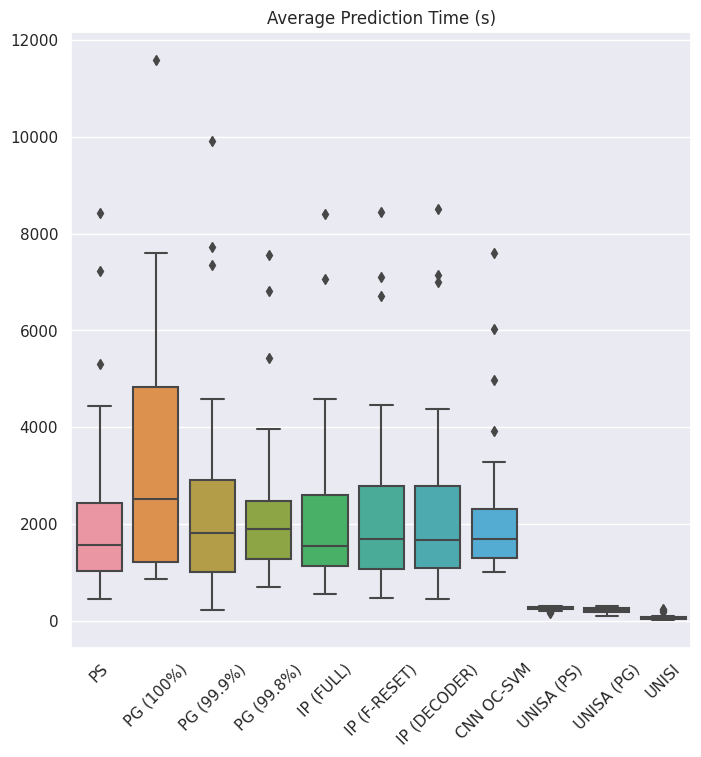
\includegraphics[width=1.0\textwidth]{images/Experimental-validation/boxplot_APT.png}
    \caption{Boxplot comparison of Average Prediction Time (s)}
    \label{fig:boxplot_APT}
\end{figure}

The average prediction times are shown in Fig. \ref{fig:boxplot_APT}. Analogous considerations to the previous case are still valid for the reference works, while the all systems trained reach a comparable median value. Once again, the best variance is achieved by the \gls{CNN} \gls{OC-SVM} work, while the worst one is obtained by the 100th percentile patient generic \gls{LSTM} based network.

The same can be said for the maximum prediction times shown in Fig. \ref{fig:boxplot_MPT}.

\begin{figure}[ht]
    \centering
    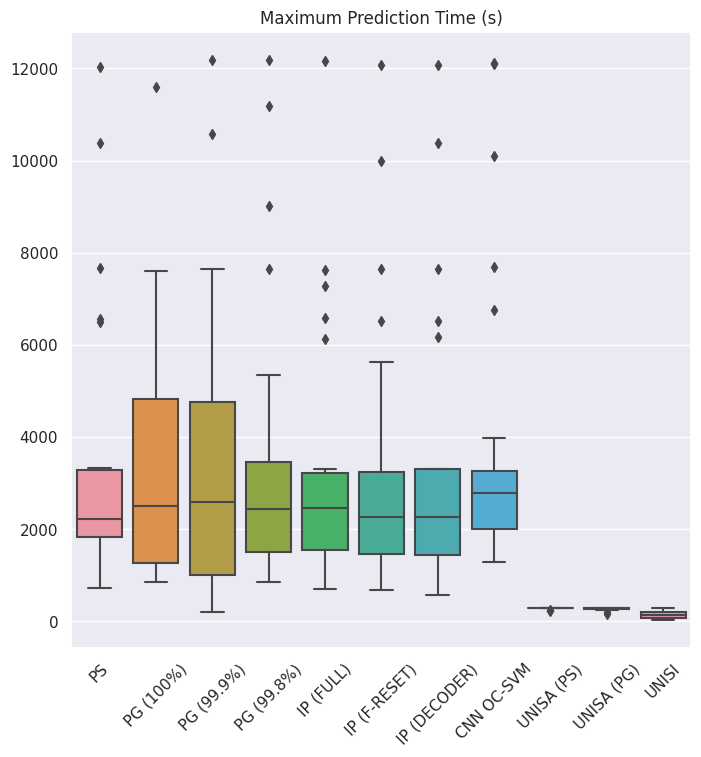
\includegraphics[width=1.0\textwidth]{images/Experimental-validation/boxplot_MPT.png}
    \caption{Boxplot comparison of Maximum Prediction Time (s)}
    \label{fig:boxplot_MPT}
\end{figure}

\clearpage
\subsection{Summary and derived metrics}
Finally, a summary of the metrics which are most interesting for real-life applicability purposes is reported in Table \ref{tab:real-life-comparison}. These results will be compared using the constraints defined the equation \ref{eq:app-constraints} as reference.

\begin{table}[ht]
    \centering
    \begin{tabular}{c|rrrrr}
    Model.  & $pred\%$ & IFP & $t_p^m$  & $\overline{t}_w$  & $t_w^M$   \\ \hline
    PS           & 39   & 162   & 1419  & 1428     & 2064     \\
    PG (100\%)   & 5    & 474   & 3887  & 823      & 825      \\
    PG (99.9\%)  & 13   & 104   & 2327  & 2786     & 3452     \\
    PG (99.8\%)  & 24   & 96    & 1708  & 2608     & 3803     \\
    IP (FULL)    & 40   & 117   & 1488  & 1950     & 2761     \\
    IP (F-RESET) & 37   & 120   & 1619  & 1974     & 2697     \\
    IP (DECODER) & 37   & 121   & 1621  & 1997     & 2740     \\
    CNN OC-SVM   & 77   & 136   & 926   & 1701     & 2936     \\
    UNISA (PS)   & 100  & 296   & 211   & 84       & 97       \\
    UNISA (PG)   & 83   & 64    & 147   & 336      & 428      \\
    UNISI        & 100  & 124   & 10    & 64       & 121      \\  \hline
    \end{tabular}
    \caption{Effective comparison between results on \glsentrylong{CHB-MIT} dataset based on real-life applicability}
    \label{tab:real-life-comparison} 
\end{table}

Among the reference works, arguably the best results are reached by \gls{UNISA}'s patient specific work: with maximum values of $pred\%$ and lowest $t_w^M$, also has acceptable values of $t_p^m$ to allow the user to hypothetically adopt safety measures when warned. Despite being the best, this system is still unusable because of its $\overline{t}_w$ and $t_w^M$, whose values approach the 100\% mark which is two orders of magnitude higher then the upper bound of 1\% pointed at in the constraints.

On the other hand, the worst reference work is the patient generic \gls{UNISA} one, with values of  $\overline{t}_w$ and $t_w^M$ well over the 100\% mark and lower values of $pred\%$.

Every reference work is still substantially better than all the developed systems.

It's hard to univocally point at the best model among those developed: while the \gls{CNN} \gls{OC-SVM} system reaches the best $pred\%$, best values of  $\overline{t}_w$ and $t_w^M$ are obtained by the 100th percentile patient generic one. However, when coupled with their relative values of $pred\%$ the best models appear to be the patient specific \gls{LSTM} based one with the lowest value of $t_w^M$ and the \gls{CNN} \gls{OC-SVM} one for its high $pred\%$, followed by the inter-patient ones for their values of $\overline{t}_w$.

\section{Evaluation of the significance of the results obtained and of the improvements that can be made}
While seizure detection is, practically, a solved problem, as also shown in the Chapter \ref{cpt:state-of-art}, not many attempts have been made towards applying unsupervised anomaly detection techniques to this task. Furthermore, the best of those few attempts achieve quite lower results, as shown in section \ref{subsec:refwork-uab}.

On the other hand, seizure prediction is much of an harder problem, with state-of-art techniques that aim to improve the everyday life of the patients, but still inevitably fail to produce usable systems.

At this point it is expected that the application of unsupervised anomaly detection techniques on seizure prediction would yield far worse results, being those techniques already unsuitable for similar, but even easier, tasks.

In spite of those unpromising assumptions, the worth of trying resides in the meaningfulness of an eventual success in the application of unsupervised anomaly detection techniques to the task of seizure prediction: as of the current state-of-art, an initial gathering of seizure instance data is mandatory, but in order to do so weeks or even months would be necessary for each patient, and that is also not taking into account the specialized medical assistance needed to gather and label those extremely long recordings. If unsupervised anomaly detection turned out to be a viable solution, the initial setup phase would require just a couple of days, and could be carried out autonomously by the patients themselves.

In the end of the analysis it is abundantly clear that the use of unsupervised anomaly detection in this reference field is \textit{not} feasible: different training approaches have been employed, such as patient specific, patient generic and inter-patient, and it was also combined with more general supervised techniques, but better results seem to be unachievable. One of the reason for such poor performance is the impossibility of enforcing a fixed preictal time during training in unsupervised scenarios, thus leading the anomaly detector to trigger as soon as an instance intrinsically anomalous is submitted: as shown in section \ref{subsec:seizure-phases}, the preictal phase is detectable as soon as 90 minutes before the seizure.

Some useful conclusion on this topic can still be made by looking at the results: the best approach is the patient specific, as also suggested by its dominance in the state-of-art, meaning that every patient has a unique manifestation of incoming seizure patterns and relative intensity, which is also confirmed by scientific literature.

In future, a system could be developed for each specific subset of patients that share the same premonitory seizure patterns, carrying out some sort of semi-supervised training which, during the first phase, would include the identification of the belonging group for that patient. One of the problems of patient specific approaches is the lack of data for the single patient, while the patient generic approach suffers from heterogeneity in seizure manifestation. This semi-supervised idea could make more data available for training while substantially limiting such variance in seizure and preictal instances.

More in general, other architectures could be tested, such as the nowadays prominent transformer which has the innate advantage of being scalable with computational power, but at the moment the amount of data in free datasets is not sufficient for taking advantage of this feature. This means that before any substantial improvement can be made, more - and possibily more specifically labeled - data must become available in the form of public datasets.